\begin{frame}{Was bisher war}
	\begin{itemize}
		\item Zwei dynamische Szenario Elemente "Pedestrian" und "Car"
		\item Ersteres für die Personenstromsimulation
		\item Letzeres für die Simulation des Kraftfahrzeugverkehrs (Felix Dietrich und Peter Zarnitz) \cite{zarnitz-2015}
	\end{itemize}
\end{frame}

\begin{frame}{Einführung des Agenten Horse}
	\begin{figure}
		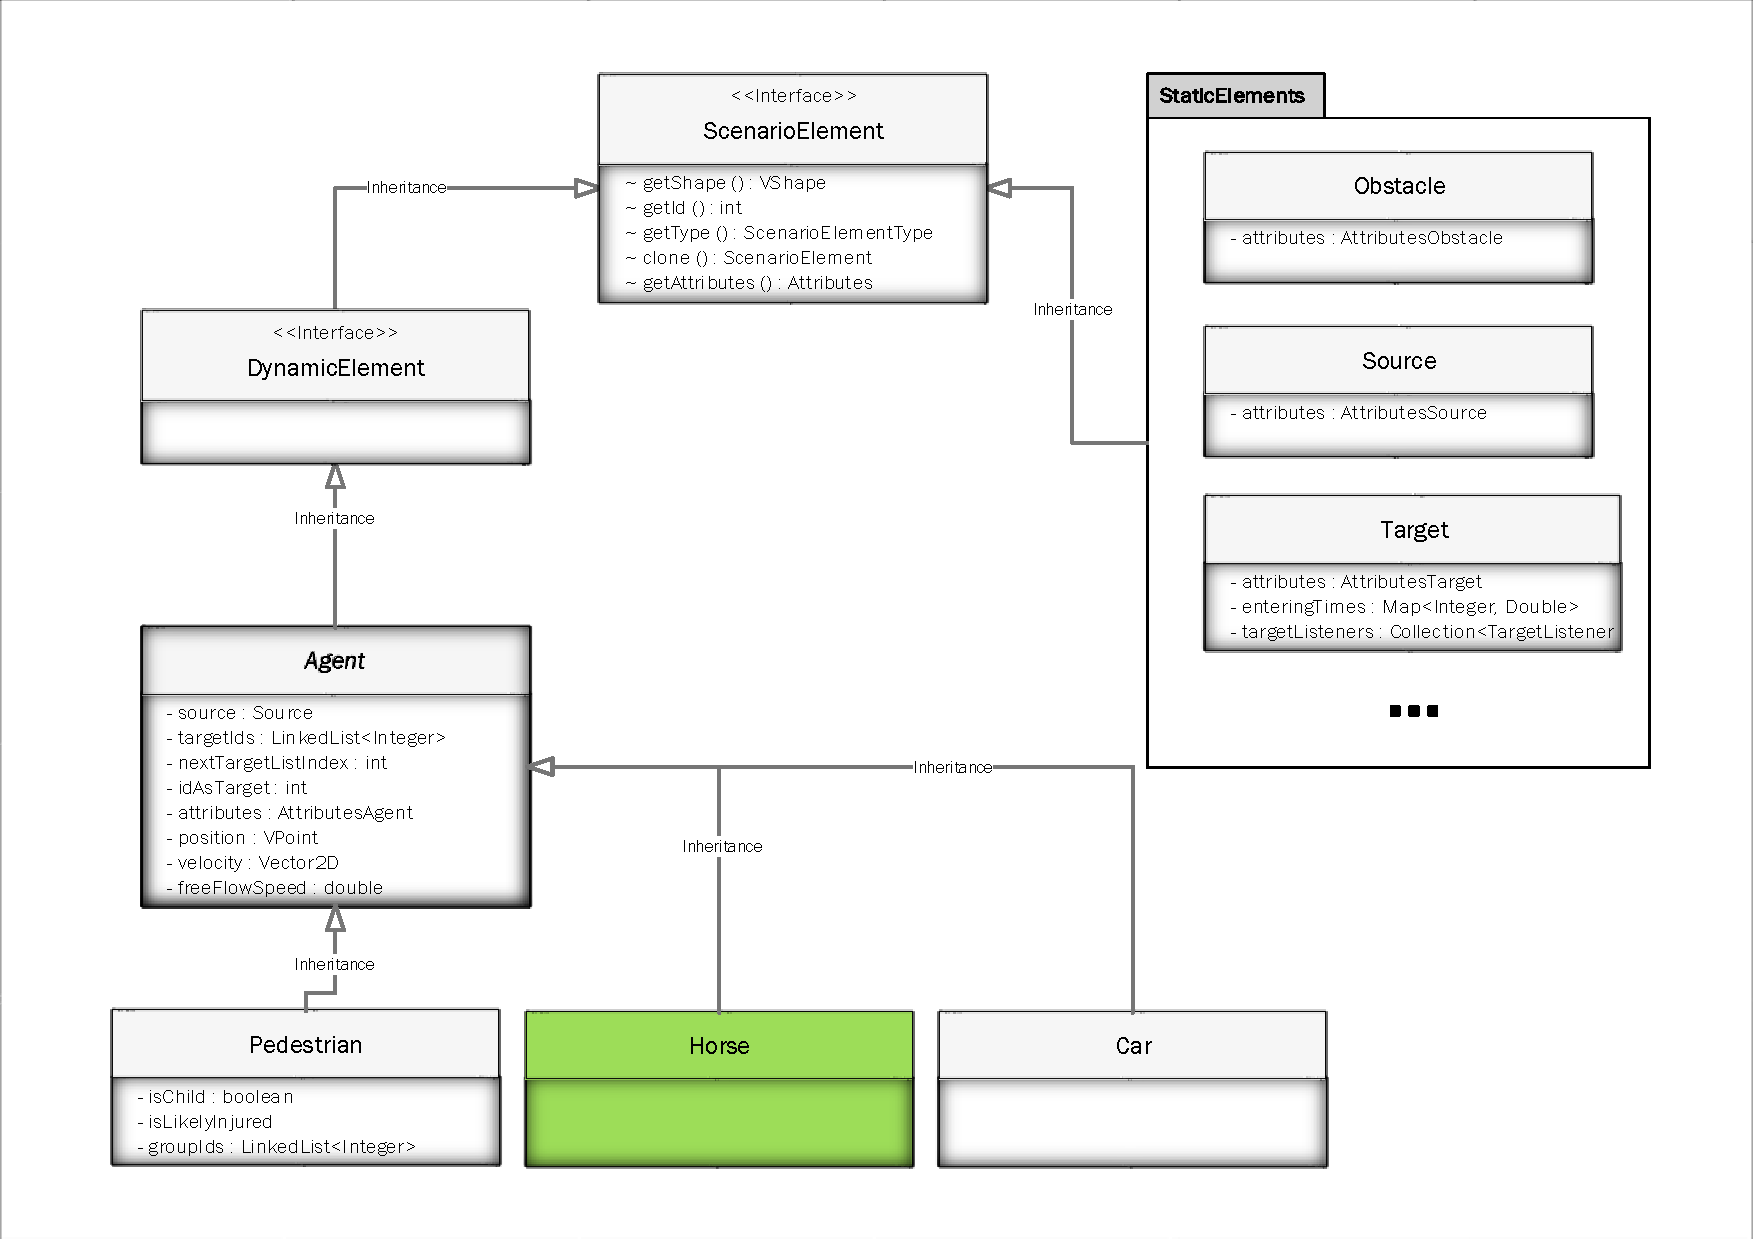
\includegraphics[width=\textwidth, keepaspectratio]{appendix/uml/ScenarioElements.pdf}
	\end{figure}
\end{frame}

\begin{frame}{Einführung des Agenten Horse}
	\begin{figure}
		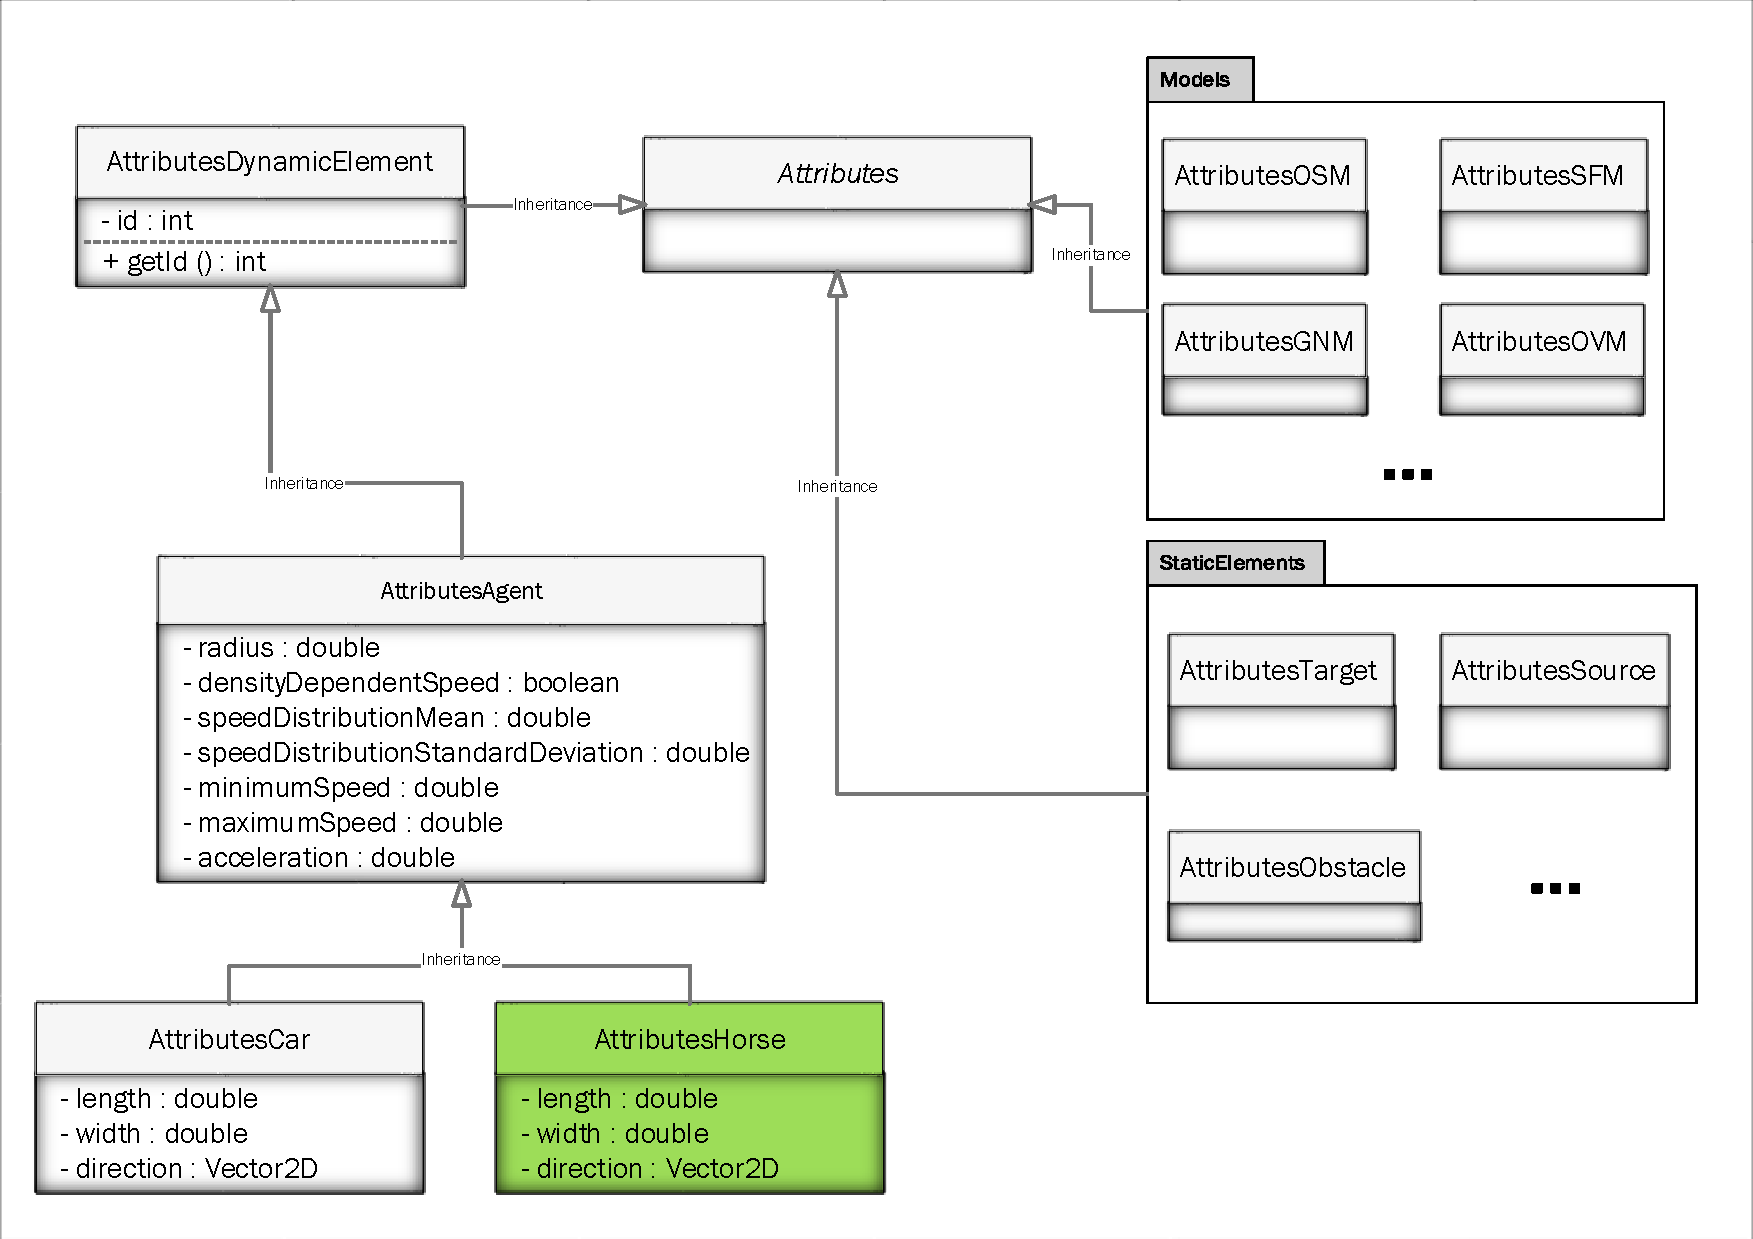
\includegraphics[width=\textwidth, keepaspectratio]{appendix/uml/Attributes.pdf}
	\end{figure}
\end{frame}

\begin{frame}{Änderungen}
	\begin{itemize}
		\item Neues dynamisches Element Horse
		\item Neuee Attribute für Horse
	\end{itemize}
\end{frame}

\begin{frame}{Review: Arbeitsaufteilung}
	\begin{figure}
		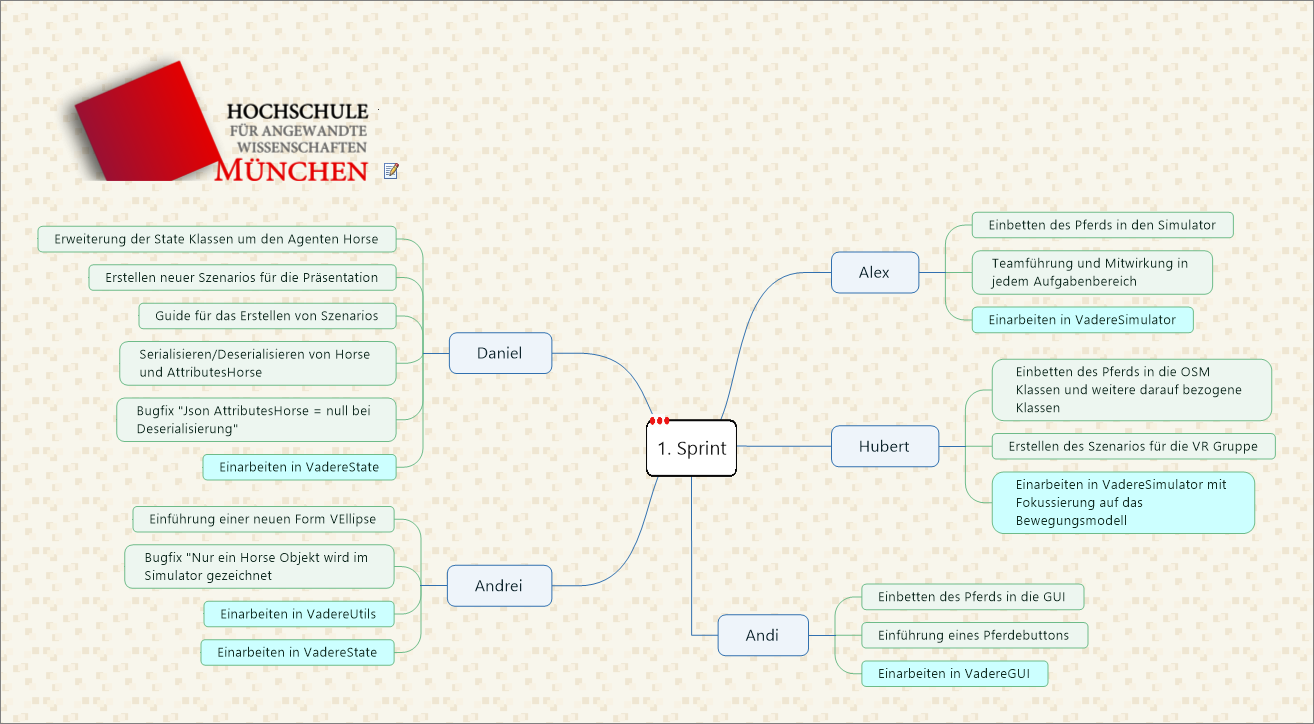
\includegraphics[width=\textwidth,keepaspectratio]{task_review.png}
	\end{figure}
\end{frame}
\begin{frame}{Ausblick}
	\begin{itemize}
		\item Bewegungsmodell des Pferdes soll entwickelt werden
		\item Bimodales Simulationsmodell für Pferd und Fußgänger
	\end{itemize}
\end{frame}
